\chapter{Build Environment}

\section{Version Numbering}

The version number of the library is provided by the \textit{safecrypto\_get\_version()} function and is represented by a 32-bit unsigned integer using the \textit{major.minor[.build[.revision]]} format. The four fields of this version numbering format are represented by 8-bit values.

\noindent The version number will be modified using the following rules:

\begin{enumerate}
\item The major version will be incremented when incompatible API changes are made.
\item The minor version number will be incremented when functionality is added in a backwards compatible manner.
\item The build version number will be incremented as development progresses and indicates that the source code has changed. When development reaches a mature level this number will be reset to $0$ and the major and/or minor version numbers will be incremented. This will typically indicate a release build.
\item The revision version number will be incremented when backwards compatible bug fixes are made to previously released builds. It will be maintained at $0$ at all other times.
\end{enumerate}

The \textit{safecrypto\_get\_version\_string()} function is used to retrieve a C string containing the version number and build date/time in a human readable form.

In addition an interface version number will be maintained as per linux library conventions (i.e. \textit{c:r:a, current, revision, age}). The first release of the library will use the interface version \textit{1:0:0}. The mechanism used to update the \textit{c:r:a} variables is defined below:

\begin{Verbatim}[commandchars=\\\{\},codes={\catcode`$=3\catcode`_=8}]
    If the interface is unchanged, but the implementation has changed or
    been fixed, then increment \textit{r}.

    Otherwise, increment \textit{c} and zero \textit{r}.

        If the interface has grown (that is, the new library is compatible
        with old code), increment \textit{a}.

        If the interface has changed in an incompatible way (that is, 
        functions have changed or been removed), then zero \textit{a}.
\end{Verbatim}


\newpage
\section{Build System}

GNU build system, also known as Autotools, is used as the build system to create distributable packages and for users to create the \textit{libsafecrypto} library, build and run example executables and run automated tests. \textbf{The development machine must have autotools, autoconf, autoconf-archive, automake, libtool, doxygen and texlive installed.}

A typical Autotools workflow as shown in Figure \ref{fig:autotools_workflow} utilises the tools \textit{Autoconf} and \textit{Automake} to generate makefiles that can be used to build a project. \textit{Autoconf} consumes the \textit{configure.ac} file to produce a shell script via the m4 macro language. This script is responsible for detecting the features and capabilities of the target system and as its name suggest it will configure the build process. \textit{Automake} consumes the \textit{Makefile.am} files to generate makefile precursors known as \textit{Makefile.in}. The configure script is responsible for converting the makefile precursors into makefiles that can be used to build the project.

\begin{figure}[H]
\centering
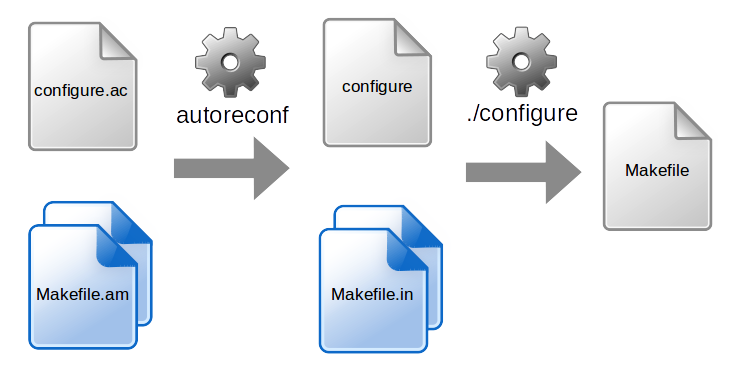
\includegraphics[width=0.6\textwidth]{autotools_workflow.png}
\caption{Autotools workflow}
\label{fig:autotools_workflow}
\end{figure}

The build system can build the design documentation (Software Coding Guidelines and Software Architecture Document) and package it into the distributable using an optional configure switch if the LaTeX tool is present on the build system. The documentation is capable of being built if the project is configured as follows:

\begin{verbatim}
    ./configure --enable-design-doc
\end{verbatim}

Unit tests are optionally built and executed if the GNU check tool is detected. All distributable packages are verified using automated unit tests. Unit tests can also be executed manually using the check target. Functional tests for the various schemes perform stress tests of the library, measure performance and exercise the major functionality of the various schemes in an effort to verify their correct operation. Functional tests are executed as part of the automated build process and must pass otherwise the build will fail in its entirety. In addition, Known Answer Tests are provided to verify the correct operation of the cryptographic schemes. All tests are executed by the build system using the \textit{check} target.

\begin{verbatim}
    make check
\end{verbatim}


\subsection{Deliverable Package}

The deliverable package is essentially the same project stored in the version control repository, the exception being the optional inclusion of pre-built design documents and the existence of a configure script.

A gzipped tarball is created by autotools for distribution and placed in the root directory of the project. This archived file is named safecrypto-x.x-x.tar.gz, using the previously mentioned development version number to uniquely identify the library.

The deliverable package is a source code package, the user must build the libraries and all associated executables. The typical process for building the libraries is as follows:

\begin{verbatim}
    ./configure [OPTIONS]
    make
    sudo make install
\end{verbatim}


\subsection{Compiler}

The GNU Compiler Collection (GCC) is used as the default compiler for the SAFEcrypto library. The library will be developed using \textbf{GCC 5.4.0} and will conform to the \textbf{C99} standard. GCC builtins will be supported by default, but a configure option and associated source code alternatives will be provided to permit the disabling of this feature.


\subsection{Compiled Library}

GNU Libtool is used to provide a consistent, portable interface for using libsafecrypto as both a static and a shared library. It removes the necessity to handle different C compilers, library functions and other low level differences between build environments by abstracting the library creation process.

The SAFEcrypto project builds the library using GNU Libtool and places it in the /libs directory at the root level. A single file is visible in this directory called libsafecrypto.la which is simply a libtool script that indicates library filenames, locations and dependencies. A hidden folder is used to store the library files themselves (i.e. /libs/.libs) as both a static archive (libsafecrypto.a) and a shared library (libsafecrypto.so.x.x.x.x) with associated symbolic links.

When the user issues a command to install the library (e.g. make install), it is the contents of the /libs folder that are installed as per the system environment. Once installed libsafecrypto can be used in the same manner as any other system installed libraries.

